
{\actuality} Жизнь многих народов Земли неразрывно связана с пещерами. В них можно найти множество полезных ресурсов, такие как металлы, драгоценные камни редкие разновидности мхов.

Но изучение пещер всегда сопровождается большими опасностями и
трудностями. К примеру таковыми являются сифоны \pic{fig:siphon}, сталактиты, обилие скользких
грунтов \pic{fig:ice}. В пещерах недостаток света и тепла, часто влажно.

Одно из преимуществ роботов --- они могут работать в опасных средах без нахождения рядом человека. Таким образом использование роботов в пещерах нивелирует все опасности для человека.

Для полноценного функционирования робота в пещере необходимы сенсоры. Классическими внешними сенсорами являются камера и лидар.

В пещерах с обилием минеральных и органических загрязнений, такие как помет летучих мышей, глина затруднительно использовать только классические способы очувствления (лидары, камеры), более того, недостаток света нивелирует преимущество классических камер из-за невозможности использования алгоритмов, где требуется большое количество фич. Типичная проблема --- грязь \pic{fig:clay} может закрыть обзор камере. Или водяной пар и водная гладь \pic{fig:splash} будут отражаться от лазера лидара и искажать полученные данные.

\begin{figure}[ht]
  \centerfloat{
      \hfill
      \subcaptionbox[List-of-Figures entry]{Сифон\label{fig:siphon}}{%
          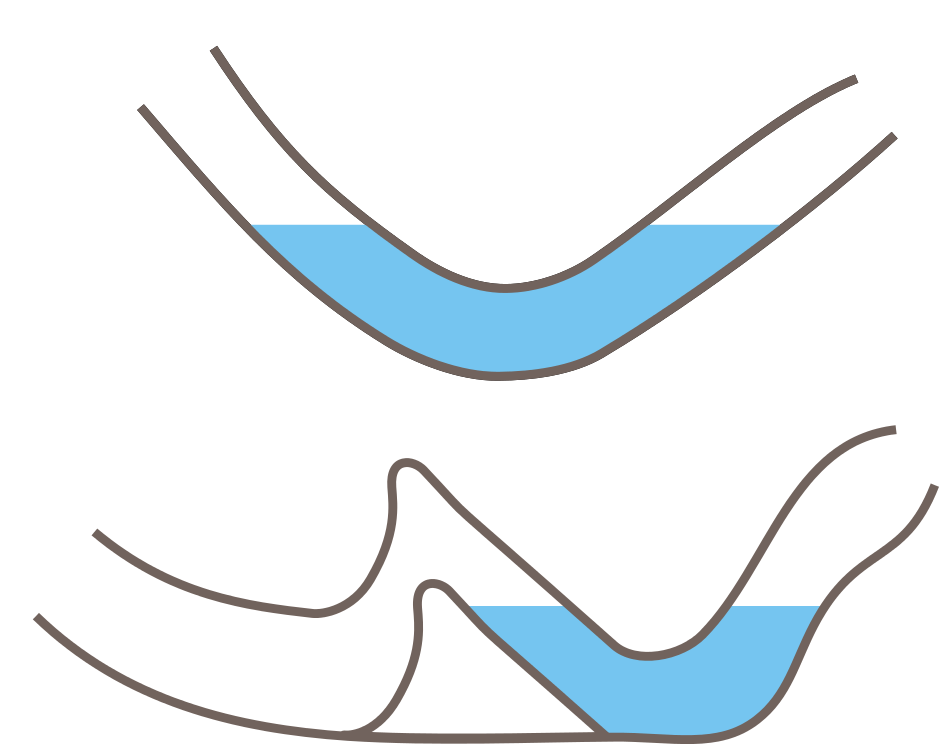
\includegraphics[width=0.24\linewidth]{surface_types/siphon.png}}
      \hfill
      \subcaptionbox{Пещера, заполненная водой по~колено\label{fig:splash}}{%
      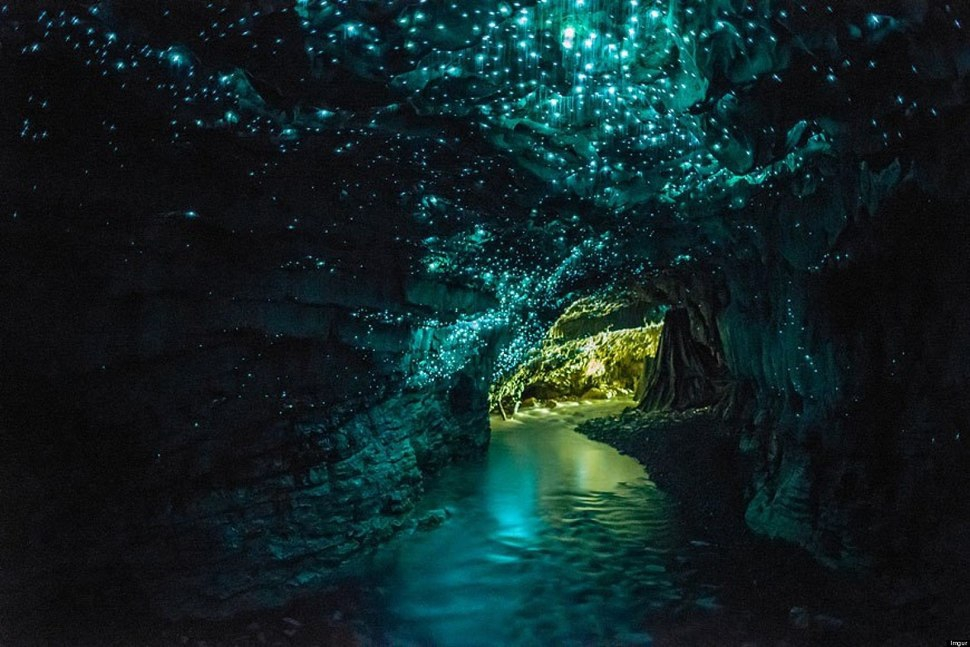
\includegraphics[width=0.24\linewidth]{surface_types/splash.png}}
      \hfill
      \subcaptionbox{Лед в пещерах\label{fig:ice}}{%
      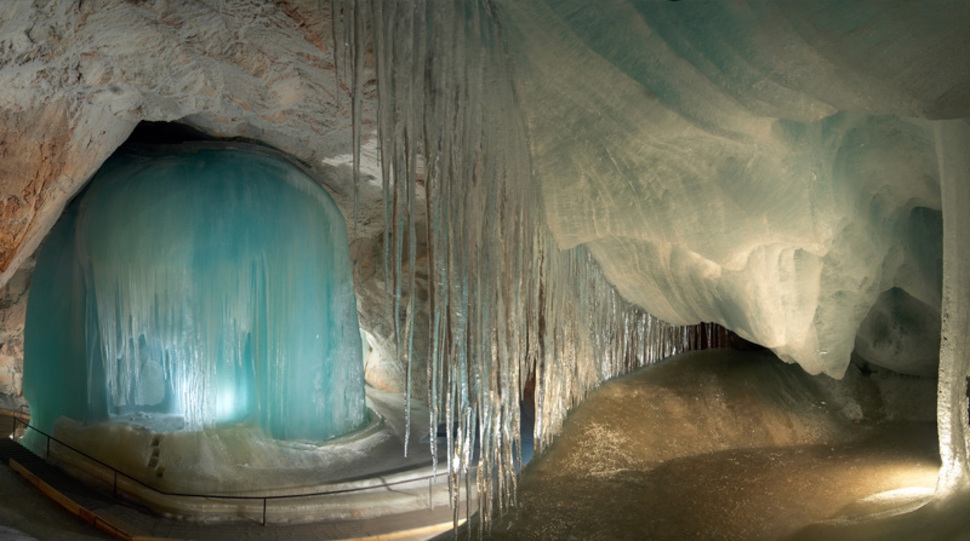
\includegraphics[width=0.24\linewidth]{surface_types/ice.png}}
      \hfill
      \subcaptionbox{Глина\label{fig:clay}}{%
          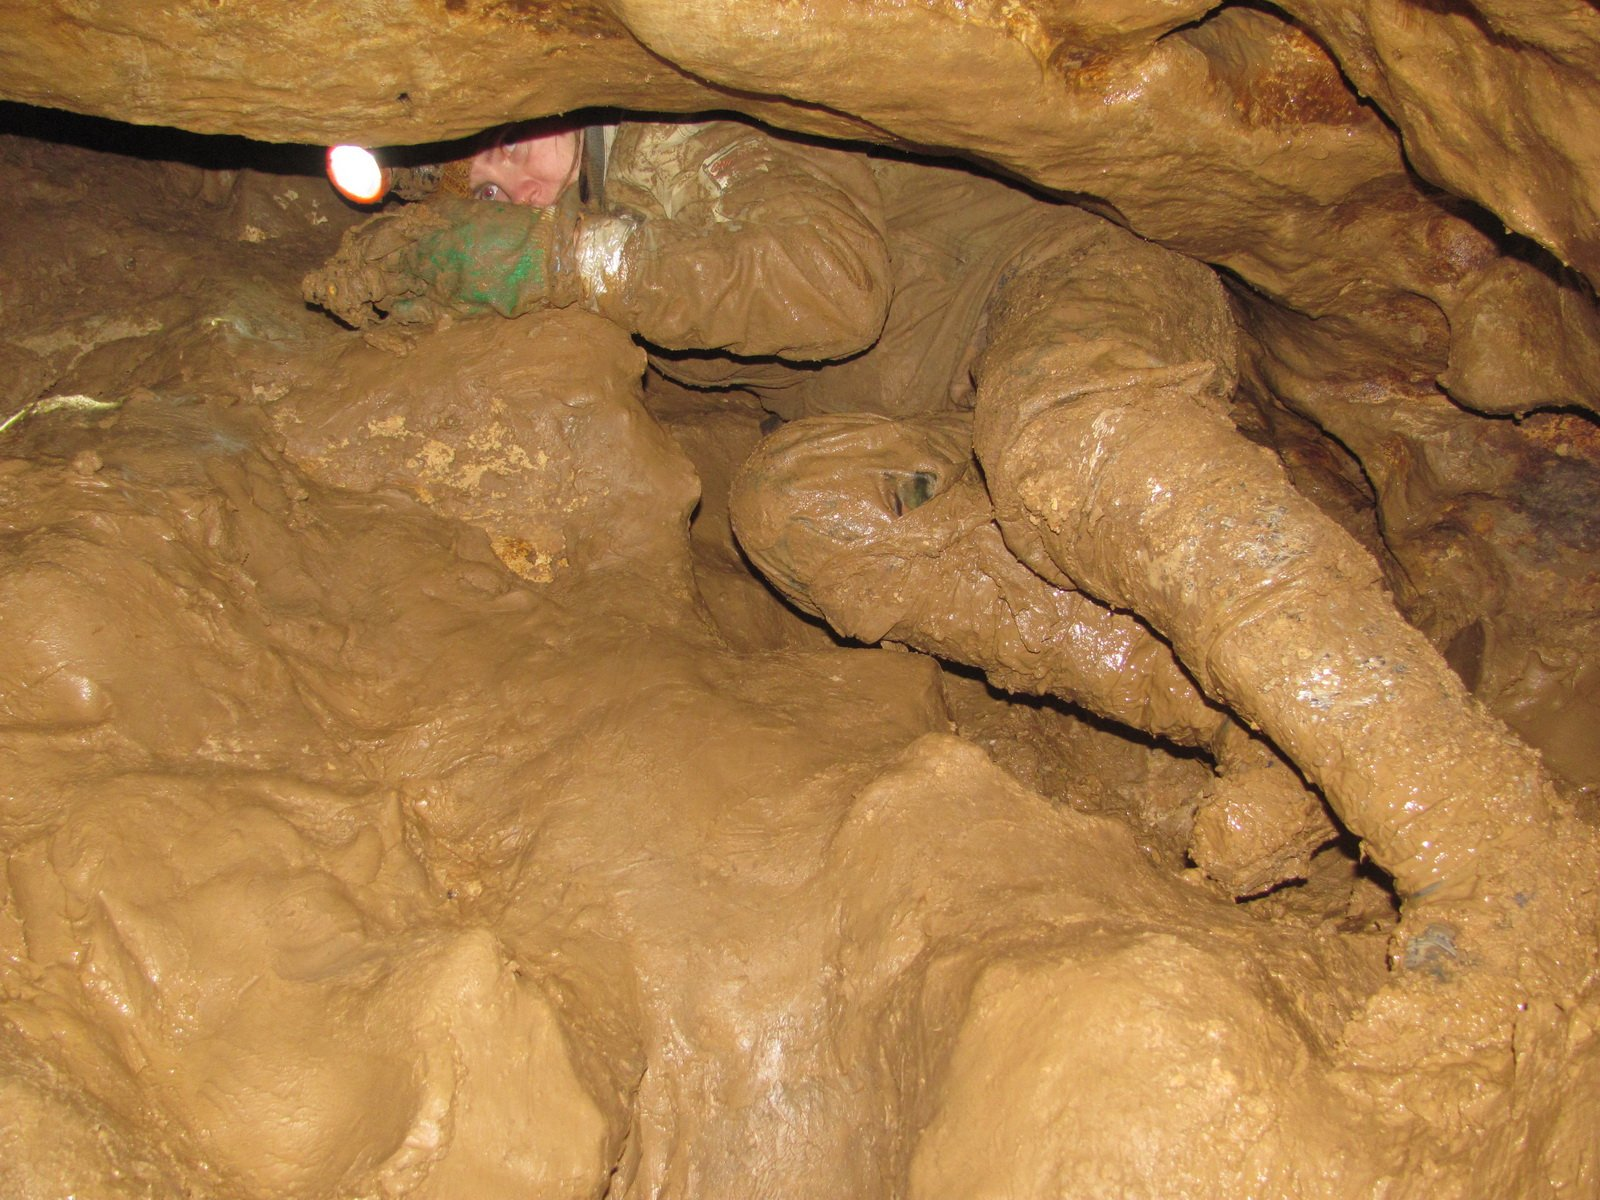
\includegraphics[width=0.24\linewidth]{surface_types/clay.jpg}}
      \hfill
  }
  % \legend{Подрисуночный текст, описывающий обозначения, например. Согласно
  %     ГОСТ 2.105, пункт 4.3.1, располагается перед наименованием рисунка.}
  \caption[Этот текст попадает в названия рисунков в списке рисунков]{Препятствия, встречающиеся в пещерах}\label{fig:obstacles}
\end{figure}
\vspace{-0.5cm}
Эту проблему возможно частично решить с помощью другого набора сенсоров. С помощью внутренних сенсоров, на которые меньше влияют внешние факторы. Такими сенсорами являются Инерциальное Измерительное устройство (IMU), датчики силы и маяки.

Таким образом необходимо разработать методику получения полезной информации об окружающей среде с помощью данного набора датчиков. Так как основные данные получаются с помощью касаний, это называется тактильным очувствлением.

Подтверждением актуальности проблемы могут являться DARPA Subterranean Challenge, отчет, который опубликовала команда Яндекс Беспилотники, а так же выделенные средства фондов НТИ и РФФИ на решение этой проблемы.

% \ifsynopsis
% Этот абзац появляется только в~автореферате.
% Для формирования блоков, которые будут обрабатываться только в~автореферате,
% заведена проверка условия \verb!\!\verb!ifsynopsis!.
% Значение условия задаётся в~основном файле документа (\verb!synopsis.tex! для
% автореферата).
% \else
% Этот абзац появляется только в~диссертации.
% Через проверку условия \verb!\!\verb!ifsynopsis!, задаваемого в~основном файле
% документа (\verb!dissertation.tex! для диссертации), можно сделать новую
% команду, обеспечивающую появление цитаты в~диссертации, но~не~в~автореферате.
% \fi

{\aim} данной работы является разработка метода тактильного очувствления мобильного шагающего робота в закрытых пространствах естественного или искусственного происхождения, в которых невозможно получение данных со спутниковой навигации, затруднено применение оптических сенсоров.

Это необходимо для проблемы получения достоверных данных о поверхности, когда робот передвигается по лужам и классические внешние сенсоры выдают некорректные данные.

Для~достижения поставленной цели необходимо было решить следующие {\tasks}:
\begin{enumerate}[beginpenalty=10000] % https://tex.stackexchange.com/a/476052/104425
  \item спроектировать объект исследования --- шагающего многоногого робота: подобрать количество ног, их форму. Обосновать конструкцию тела и количество степеней свободы;
  \item подобрать сенсоры для решения поставленной задачи;
  \item разработать методику построения карты местности и определения типа поверхности с помощью тактильного очувствления;
  \item решить проблему локализации на основе тактильного очувствления.
\end{enumerate}

{\researchobj}
Для разведки местности под землей в труднодоступных местах с малой видимостью разработан прототип многоногого шагающего робота СтриРус \pic{fig:strirus_4}

Данный робот состоит из двух сегментов с одной активной степенью свободы. Робот обладает 10 независимыми лапками, 6 лап в первом сегменте и 4 во втором.

Особенность конструкции робота в том, что возможно изменять угол между лапкой и корпусом робота. Данное конструктивное изменение позволило сделать перемещение робота всенаправленным, то есть робот может двигаться во все стороны без смены ориентации корпуса робота.


{\methods} За базис были взяты методологии из теории робототехнических систем, теоретической механики, механизмов и машин, теории оптимизации.

Для экспериментального исследования применялось численное и стендовое моделирования.

{\reliability} Правдивость результатов обеспечивается согласованностью с опубликованными результатами научных исследований других авторов, подтверждаются результатами компьютерного моделирования, натурными испытаниями. Результаты диссертационного исследования докладывались и обсуждались на российских и международных научных конференциях, и получили положительный отзыв научной общественности.


{\novelty} состоит в формулировании проблемы построения карты с помощью тактильного очувствления, а так же ее комплексного решения. В это решение входит разработка метода оптимизации конструкции робота, методика исследования датчика силы, а так же методика построения карты местности с помощью датчиков силы, установленных на ногах робота.

\textbf{Доказана} возможность построения карты местности и определения типа поверхности с помощью тактильного очувствления как в робототехническом симуляторе, так с помощью натурного эксперимента.

\textbf{Показано}, что оптимальное количество ног для циклового движителя с одной степенью свободы в ноге находится в диапазоне от 8 до 14 ног. 

\textbf{Предложено} использовать преобразователь силы на основе полимерного материала Velostat. \textbf{Установлено}, что данный преобразователь можно рассматривать как единое тело, при площади нажатия больше 50\% площади сенсора. 

\textbf{Сделан вывод} об эффективности предложенных методик, на основе результатов натурных испытаний.

{\defpositions}
\begin{enumerate}[beginpenalty=10000] % https://tex.stackexchange.com/a/476052/104425
  \item метод оптимизации конструкции многоногих роботов;
  \item разработанная методика исследования датчика силы, когда площадь нажатия на сенсор меньше самого сенсора;
  \item реализация программно-алгоритмического обеспечения (ПАО), позволяющего определять тип поверхности;
  \item методика построения карты местности с помощью датчиков силы, установленных на ногах робота.
\end{enumerate}


{\influence} Реализация полученных результатов в виде продукта позволит получить надежную резервную систему навигации для робота, у которого есть датчики силы, IMU и возможность устанавливать маяки по мере продвижения.

Если у робота есть только датчики силы, будет возможно получать информацию о типе пройденной поверхности, а так же строить карту поверхности под толщей воды, там где лидар и камера не смогут выдать адекватный результат.


{\probation}
Основные результаты работы докладывались~на:
\begin{itemize}
  \item ICINCO 2017 --- 14th International Conference on Informatics in Control, Automation and Robotics (Madrid, Spain, 26-28 july 2017);
  \item IEEE International Conference on Robotics and Biomimetics, ROBIO 2017 (Macau, China, 5-8 december 2017);
  \item  международной  научно-практической  конференции  «Прогресс  транспортных 
  средств и систем» (г. Волгоград, 9-11 октября 2018 г.);
  \item 23rd IEEE FRUCT Conference (Bologna, Italy, 13-16 november 2018).
  \item XXXI международной конференции молодых ученых и студентов МИКМУС-2019 
  (г. Москва, 4-6 декабря 2019 г.);
  \item Международная конференция <<Зимняя Школа Робототехники в Сириусе --- 2022>> (г. Адлер, Россия, 25 января - 6 февраля 2022)
\end{itemize}

{\contribution} Все научные результаты диссертации, выдвигаемые для защиты, получены автором лично.

% Вставка кто сколько опубликовался
\ifnumequal{\value{bibliosel}}{0}
{%%% Встроенная реализация с загрузкой файла через движок bibtex8. (При желании, внутри можно использовать обычные ссылки, наподобие `\cite{vakbib1,vakbib2}`).
    {\publications} Основные результаты по теме диссертации изложены
    в~XX~печатных изданиях,
    X из которых изданы в журналах, рекомендованных ВАК,
    X "--- в тезисах докладов.
}%
{%%% Реализация пакетом biblatex через движок biber
    \begin{refsection}[bl-author, bl-registered]
        % Это refsection=1.
        % Процитированные здесь работы:
        %  * подсчитываются, для автоматического составления фразы "Основные результаты ..."
        %  * попадают в авторскую библиографию, при usefootcite==0 и стиле `\insertbiblioauthor` или `\insertbiblioauthorgrouped`
        %  * нумеруются там в зависимости от порядка команд `\printbibliography` в этом разделе.
        %  * при использовании `\insertbiblioauthorgrouped`, порядок команд `\printbibliography` в нём должен быть тем же (см. biblio/biblatex.tex)
        %
        % Невидимый библиографический список для подсчёта количества публикаций:
        \printbibliography[heading=nobibheading, section=1, env=countauthorvak,          keyword=biblioauthorvak]%
        \printbibliography[heading=nobibheading, section=1, env=countauthorwos,          keyword=biblioauthorwos]%
        \printbibliography[heading=nobibheading, section=1, env=countauthorscopus,       keyword=biblioauthorscopus]%
        \printbibliography[heading=nobibheading, section=1, env=countauthorconf,         keyword=biblioauthorconf]%
        \printbibliography[heading=nobibheading, section=1, env=countauthorother,        keyword=biblioauthorother]%
        \printbibliography[heading=nobibheading, section=1, env=countregistered,         keyword=biblioregistered]%
        \printbibliography[heading=nobibheading, section=1, env=countauthorpatent,       keyword=biblioauthorpatent]%
        \printbibliography[heading=nobibheading, section=1, env=countauthorprogram,      keyword=biblioauthorprogram]%
        \printbibliography[heading=nobibheading, section=1, env=countauthor,             keyword=biblioauthor]%
        \printbibliography[heading=nobibheading, section=1, env=countauthorvakscopuswos, filter=vakscopuswos]%
        \printbibliography[heading=nobibheading, section=1, env=countauthorscopuswos,    filter=scopuswos]%
        %
        \nocite{*}%
        %
        {\publications} Основные результаты по теме диссертации изложены в~\arabic{citeauthor}~печатных изданиях,
        \arabic{citeauthorvak} из которых изданы в журналах, рекомендованных ВАК\sloppy%
        \ifnum \value{citeauthorscopuswos}>0%
            , \arabic{citeauthorscopuswos} "--- в~периодических научных журналах, индексируемых Web of~Science и Scopus\sloppy%
        \fi%
        \ifnum \value{citeauthorconf}>0%
            , \arabic{citeauthorconf} "--- в~тезисах докладов.
        \else%
            .
        \fi%
        \ifnum \value{citeregistered}=1%
            \ifnum \value{citeauthorpatent}=1%
                Зарегистрирован \arabic{citeauthorpatent} патент.
            \fi%
            \ifnum \value{citeauthorprogram}=1%
                Зарегистрирована \arabic{citeauthorprogram} программа для ЭВМ.
            \fi%
        \fi%
        \ifnum \value{citeregistered}>1%
            Зарегистрированы\ %
            \ifnum \value{citeauthorpatent}>0%
            \formbytotal{citeauthorpatent}{патент}{}{а}{}\sloppy%
            \ifnum \value{citeauthorprogram}=0 . \else \ и~\fi%
            \fi%
            \ifnum \value{citeauthorprogram}>0%
            \formbytotal{citeauthorprogram}{программ}{а}{ы}{} для ЭВМ.
            \fi%
        \fi%
        % К публикациям, в которых излагаются основные научные результаты диссертации на соискание учёной
        % степени, в рецензируемых изданиях приравниваются патенты на изобретения, патенты (свидетельства) на
        % полезную модель, патенты на промышленный образец, патенты на селекционные достижения, свидетельства
        % на программу для электронных вычислительных машин, базу данных, топологию интегральных микросхем,
        % зарегистрированные в установленном порядке.(в ред. Постановления Правительства РФ от 21.04.2016 N 335)
    \end{refsection}%
    \begin{refsection}[bl-author, bl-registered]
        % Это refsection=2.
        % Процитированные здесь работы:
        %  * попадают в авторскую библиографию, при usefootcite==0 и стиле `\insertbiblioauthorimportant`.
        %  * ни на что не влияют в противном случае
        \nocite{vakbib2}%vak
        \nocite{patbib1}%patent
        \nocite{progbib1}%program
        \nocite{bib1}%other
        \nocite{confbib1}%conf
    \end{refsection}%
        %
        % Всё, что вне этих двух refsection, это refsection=0,
        %  * для диссертации - это нормальные ссылки, попадающие в обычную библиографию
        %  * для автореферата:
        %     * при usefootcite==0, ссылка корректно сработает только для источника из `external.bib`. Для своих работ --- напечатает "[0]" (и даже Warning не вылезет).
        %     * при usefootcite==1, ссылка сработает нормально. В авторской библиографии будут только процитированные в refsection=0 работы.
}
% При использовании пакета \verb!biblatex! будут подсчитаны все работы, добавленные
% в файл \verb!biblio/author.bib!. Для правильного подсчёта работ в~различных
% системах цитирования требуется использовать поля:
% \begin{itemize}
%         \item \texttt{authorvak} если публикация индексирована ВАК,
%         \item \texttt{authorscopus} если публикация индексирована Scopus,
%         \item \texttt{authorwos} если публикация индексирована Web of Science,
%         \item \texttt{authorconf} для докладов конференций,
%         \item \texttt{authorpatent} для патентов,
%         \item \texttt{authorprogram} для зарегистрированных программ для ЭВМ,
%         \item \texttt{authorother} для других публикаций.
% \end{itemize}
% Для подсчёта используются счётчики:
% \begin{itemize}
%         \item \texttt{citeauthorvak} для работ, индексируемых ВАК,
%         \item \texttt{citeauthorscopus} для работ, индексируемых Scopus,
%         \item \texttt{citeauthorwos} для работ, индексируемых Web of Science,
%         \item \texttt{citeauthorvakscopuswos} для работ, индексируемых одной из трёх баз,
%         \item \texttt{citeauthorscopuswos} для работ, индексируемых Scopus или Web of~Science,
%         \item \texttt{citeauthorconf} для докладов на конференциях,
%         \item \texttt{citeauthorother} для остальных работ,
%         \item \texttt{citeauthorpatent} для патентов,
%         \item \texttt{citeauthorprogram} для зарегистрированных программ для ЭВМ,
%         \item \texttt{citeauthor} для суммарного количества работ.
% \end{itemize}
% % Счётчик \texttt{citeexternal} используется для подсчёта процитированных публикаций;
% % \texttt{citeregistered} "--- для подсчёта суммарного количества патентов и программ для ЭВМ.

% Для добавления в список публикаций автора работ, которые не были процитированы в
% автореферате, требуется их~перечислить с использованием команды \verb!\nocite! в
% \verb!Synopsis/content.tex!.


Диссертационная работа была выполнена при поддержке грантов:
\begin{itemize}
    \item НТИ по поддержке Центра <<Технологий Компонентов Робототехники и Мехатроники>> на базе Университета Иннополис по теме <<Разработка роботизированных платформ для автономной подземной и наземной инспекции местности в условиях трудной проходимости и плохой видимости>>. 
    \item РФФИ № 20-38-90265 по теме <<Разработка метода очувствления мобильного шагающего робота, перемещающегося в закрытом пространстве естественного происхождения>>.
\end{itemize}

{\struct}
В введении рассказывается об актуальности проблемы, в чем научная новизна и цель проекта.

Во первой главе показан обзор существующих решений.

Вторая глава покрывает разработку объекта исследования, а именно решение задачи топологического синтеза и инженерную разработку прототипа.

Третья глава посвящена разработке и исследованию самодельного преобразователя силы на основе Velostat.

Четвертая глава раскрывает детали создания алгоритма построения карты с помощью тактильного очувствления, решение проблемы локализации с помощью датчиков датчиков силы, IMU и маяков. Решатся проблема определения типа поверхности.